\section{The Aphetic Points/Transmissions (11K,7P)}

The aphetic points of the years are operative when starting from any star, but the following aphetic points are most effective: for day births the \Sun, for night births the \Moon, especially when they are at the
angles. Next $<$in effectiveness$>$ is the Ascendant. 

If the vital sector starting from the Ascendant, the \Moon, or the \Sun\xspace passes to one of the stars in the nativity, then use it for forecasting. If one of the stars in transit has entered this place, then it will be transmitting the chroncratorship. If the sign where the count stops happens to be empty, then count from the position (at the nativity) of the ruler of the sign, and examine in the same way the place found, whether using the nativity or the transiting stars. Then forecast the results of all the places and stars. $<$In other words,$>$ if the count goes from star to star, use the stars for forecasting; if
from a star to an empty sign, use the rulers of the signs.

An example: if the aphetic point goes from the moon to either \Aries\xspace or \Scorpio, \textbf{/221P/} but no stars are
in either sign, then count off the same number of years from the position of \Mars\xspace $<$ruler of \Aries\xspace and \Scorpio$>$ at the nativity; if the count stops at \Saturn, the year will be dangerous and troublesome, plus whatever else the transmissions and the places indicate. The same method holds true for the year starting from the \Sun, the Ascendant, or the Lots: each will forecast an appropriate result according to its transmission and reception.

Now if two stars are active in one year, $<$both transmissions will be effective$>$, but especially those from the angles, next those from signs which follow the angles, next those from signs which precede the angles. 

Benefics transmitting or receiving from angles, exaltations, or operative places become the cause of great good and high rank; when transmitting or receiving from signs which follow the angles, they cause moderate good; when transmitting and receiving from signs which precede the angles, they are weak. When transmitting or receiving from $<$signs$>$ in opposition, they are damaging and troublesome. 

In the same way malefics acting at the angles are the worst; in signs which follow the angles they are mediocre and bring crises slowly; in signs which precede the angles they are less bad. When acting in opposition they are indicative of reversals and dangers.

\textbf{/233K/} Whenever malefics in superior aspect receive the chronocratorship from stars in inferior aspect, they make the bad even worse, even if they are in opposition to benefics and are receiving from them. When trine $<$with benefics$>$ they make their results more agreeable and mild. 

The receivers are considered more influential than the transmitters: it is better if a benefic transmits to a benefic than if a malefic transmits to a benefic; it is the worst if a malefic transmits to a malefic. 

If the vital sector comes to a currently empty sign, but later a star transits this place, that star will be receiving the chronocratorship. A
star’s influence will be considered very vigorous, whether benefic or malefic, if it is passing through a phase in that sign; if it is transiting, it is weak. If the vital sector comes to an empty sign, the vital sector of the previous year $<$=chronocratorship$>$ will have the control until another takes effect.

The settings and retrograde periods of the stars will be weak, the risings and stationary points will be vigorous, blending their influences in complex ways. $<$Forecast$>$ according to the basis of the nativity for the rich, the middle class, the toilers, the poor, and the craftsmen.

Forecasts will be quite definite with respect to actions and critical points when the same stars come into the same configuration they had at the nativity—as the divine Critodemus reminds us. We append his system in the following chart and the accompanying directions: \textbf{/222P/}

\begin{small}
\begin{longtable}[c]{c|c c c c c c c c c c c c}
\caption{Critodemus' System [Profection Sign Intervals]}
\label{Table 5.2} \\
\hline
 & \Aries & \Taurus & \Gemini & \Cancer & \Leo & \Virgo
 & \Libra &  \Scorpio & \Sagittarius & \Capricorn & \Aquarius & \Pisces 
 \\
\hline
\endhead
\Aries & 1 & 12 & 11 & 10 & 9 & 8 & 7 & 6 & 5 & 4 & 3 & 2 \\
\Taurus & 2 & 1 & 12 & 11 & 10 & 9 & 8 & 7 & 6 & 5 & 4 & 3 \\
\Gemini & 3 & 2 & 1 & 12 & 11 & 10 & 9 & 8 & 7 & 6 & 5 & 4 \\
\Cancer & 4 & 3 & 2 & 1 & 12 & 11 & 10 & 9 & 8 & 7 & 6 & 5 \\
\Leo & 5 & 4 & 3 & 2 & 1 & 12 & 11 & 10 & 9 & 8 & 7 & 6 \\
\Virgo & 6 & 5 & 4 & 3 & 2 & 1 & 12 & 11 & 10 & 9 & 8 & 7 \\
\Libra & 7 & 6 & 5 & 4 & 3 & 2 & 1 & 12 & 11 & 10 & 9 & 8 \\
\Scorpio &  8 & 7 & 6 & 5 & 4 & 3 & 2 & 1 & 12 & 11 & 10 & 9 \\
\Sagittarius & 9 & 8 & 7 & 6 & 5 & 4 & 3 & 2 & 1 & 12 & 11 & 10 \\
\Capricorn & 10 & 9 & 8 & 7 & 6 & 5 & 4 & 3 & 2 & 1 & 12 & 11 \\
\Aquarius & 11 & 10 & 9 & 8 & 7 & 6 & 5 & 4 & 3 & 2 & 1 & 12 \\
\Pisces & 12 & 11 & 10 & 9 & 8 & 7 & 6 & 5 & 4 & 3 & 2 & 1 \\
\hline
\end{longtable}
\end{small}

The preceding table is the table of the stars’ mutual return to the same intervals and configurations. 

\newpage
\begin{wrapfigure}[15]{R}{7cm}
\centering
\vspace{0pt}
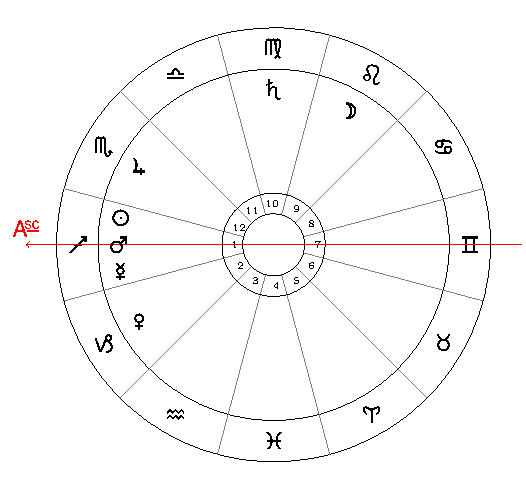
\includegraphics[width=.68\textwidth]{charts/5_11_1}
\caption{Chart 69 [V.11.1, GH L37]}
\label{fig:chart69}
\end{wrapfigure}

\noindent For example: \Sun, \Mars, \Mercury, Ascendant in \Sagittarius, \Moon\xspace in \Leo, \Saturn\xspace in \Virgo, \Jupiter\xspace in \Scorpio, \Venus\xspace in \Capricorn\footnote{\textit{Greek Horoscopes} dates the chart to December 15, 37 CE about sunrise}. 

The \Moon\xspace controls the second interval since it is two signs from \Saturn. The same is true of the \Sun, \Mars, \Mercury, and the Ascendant with respect to \Venus. \Saturn, \Jupiter, and \Venus\xspace control the third interval. \Saturn\xspace controls the fourth and fifth interval. The \Moon\xspace controls the sixth. The seventh is common to all. \Venus\xspace controls the eighth. The \Sun, \Mars, \Mercury, and the Ascendant the ninth. Jupiter the tenth and eleventh, and \Venus\xspace the twelfth. 

The horoscope is in its 31st year. The operative stars and the critical points are found as follows: when calculating the previously mentioned critical points, begin at \textbf{/234K/} the third row (=third interval), because the preceding two intervals, the first and the second, are inoperative. (The first is operative to year 12, the second to year 24,
the third to year 36, and so on.) It is calculated thus: since the 31st year falls in the eleventh column of the third interval, and since \Saturn, \Jupiter, and \Venus\xspace control the third interval at the nativity, investigate the stars \textbf{/223P/} in transit at the time in question to see if they transmit to another star or to themselves at a
distance of 11 signs. 

Take the preceding nativity: the stars’ positions at the time in question were as follows: \Sun, \Jupiter, \Mercury\xspace in \Gemini, \Saturn\xspace in \Virgo, \Mars, \Venus\xspace in \Taurus, \Moon\xspace in \Pisces. Now the stars controlling the interval of 11 were \Saturn, \Jupiter, and \Venus, and we find at the time in question
that \Venus\xspace has returned to a position 11 signs from the \Moon, but that no star has returned to a position 11 signs from \Jupiter. Immediately I move to the fourth row. I find 32 in the eighth position. None of the ruling stars are critical in the fourth interval. I move to the fifth interval: the \Moon\xspace and \Saturn\xspace are operative
in the fifth interval and are found to be returning to each other five signs apart. I move to the sixth interval: no stars are six signs apart. I move to the row of the seventh interval. [The chronocratorship is found to be passing through the fifth interval.] The seventh interval is found to be empty of any star (as mentioned above); \Mars\xspace and \Venus\xspace to \Saturn\xspace $<$?$>$. I move to the row of the eighth interval: \Venus\xspace rules the eighth interval because of the factor 4. It is returning to no star. Then to the critical point of the ninth interval: the \Sun, \Mars, \Mercury, the Ascendant, and \Venus\xspace rule the ninth interval; 36 is in this row. 

At a 4-year interval the \Sun, \Jupiter, and \Mercury\xspace are found to be returning to \Saturn. Next I move to the tenth interval: the \Sun,\Mars, \Mercury, \Jupiter, and the Ascendant rule the tenth; in this row is the number 4; therefore the \Sun, \Mercury, and \Jupiter\xspace are found to be transmitting to \Saturn.

The chronocrators found by using these intervals will be incontrovertibly active and operative when their rulers at the nativity have the same intervals in their transits at the time in question as they had at the
nativity.
\newpage